\section{Methodology}
\begin{figure}
    \centering
    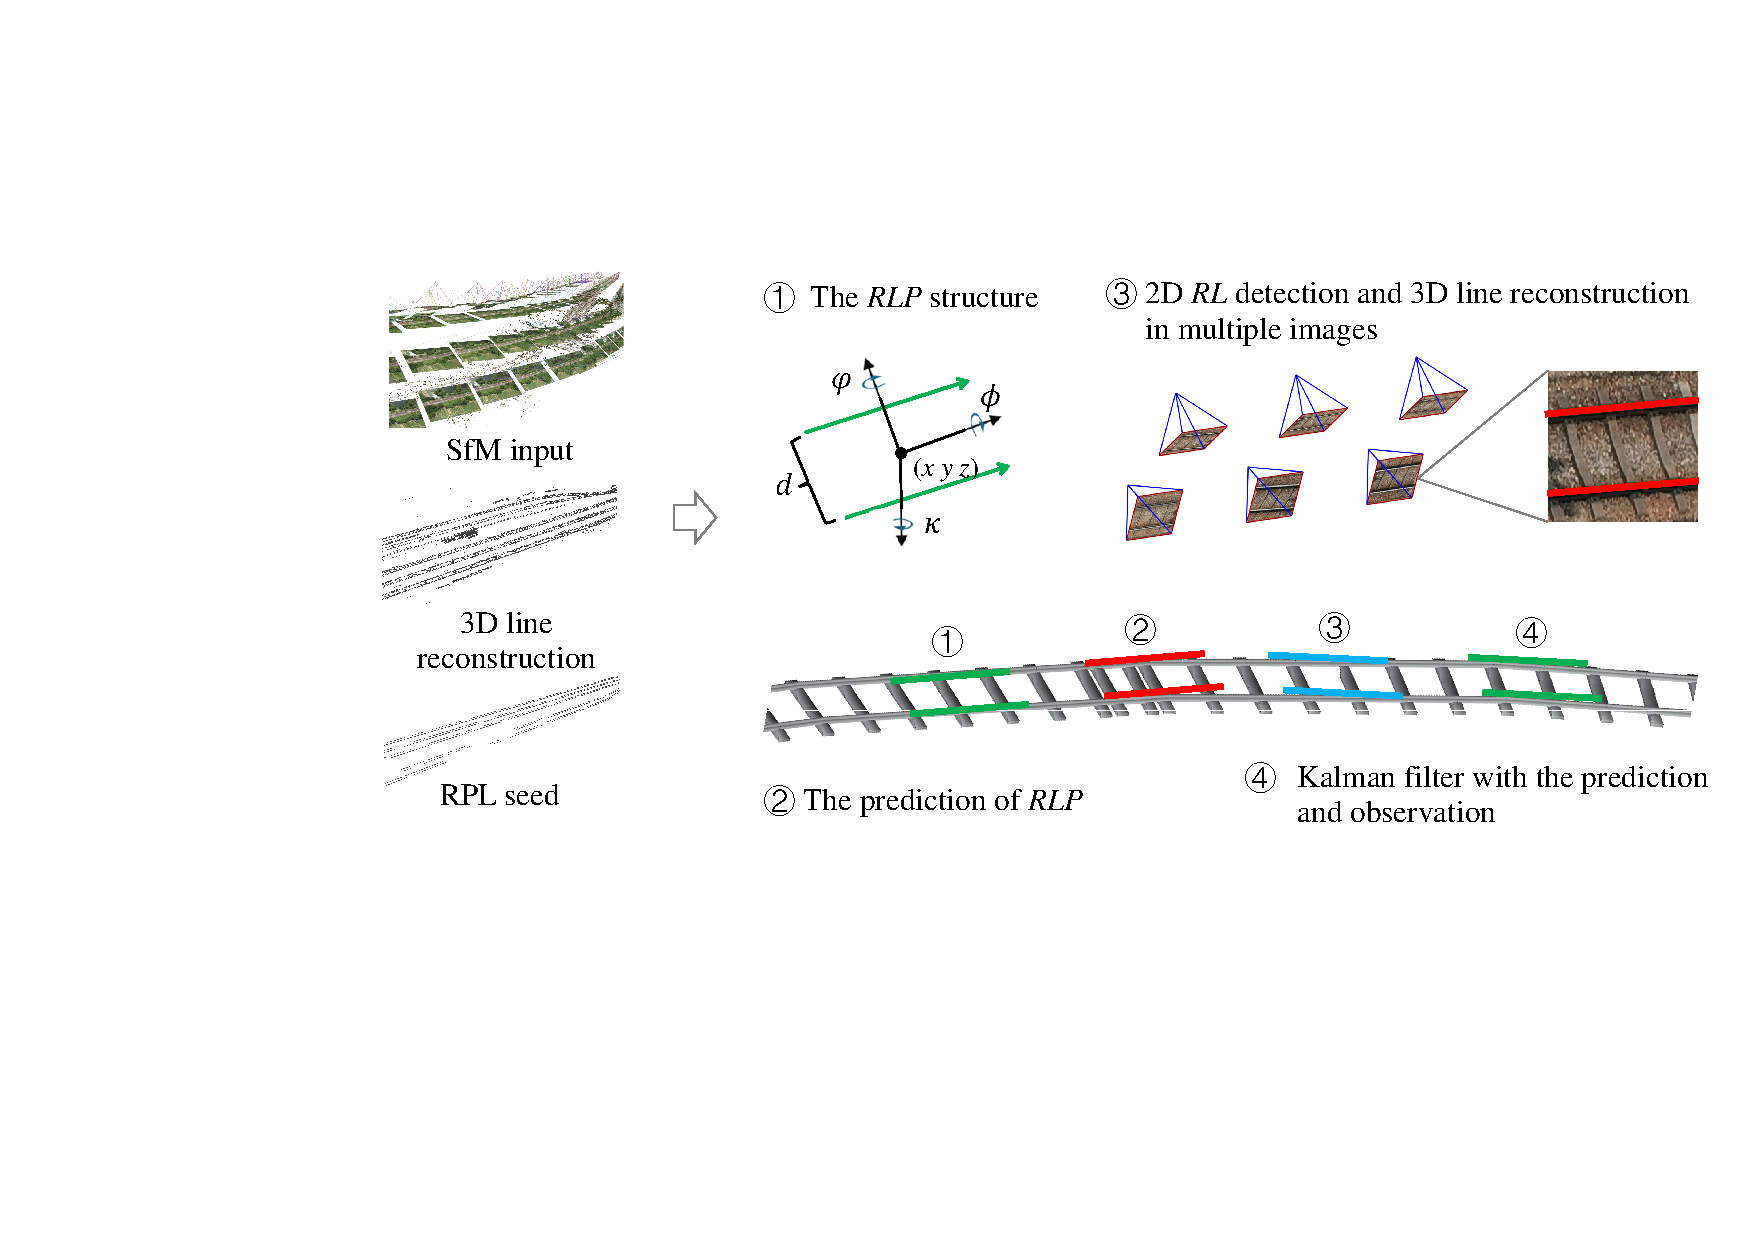
\includegraphics[width=0.98\textwidth]{images/overview.pdf}
    \caption{The flow of our method.
    It uses the aerial images as the input and produces accurate
    and connected 3D railway lines.}
    \label{fig_overview}
\end{figure}

The flow is presented in \cref{fig_overview}.
The basic cell of our reconstruction is the railway line pair (\rlp) consisting of two railway lines (\textit{RL})~(\cref{fig_overview}~(1)).
We use a center point $\mathbf p=\left(x,y,z\right)$,
the forward vector $\mathbf d=\left(d_x,d_y,d_z\right)$,
the rotation angle $r$ perpendicular to $\mathbf d$,
and the with $w$ to shape the \rlp:
\begin{equation}
\mathbf x = \begin{bmatrix}
    \mathbf p  & \mathbf d  & \mathbf d_2 
\end{bmatrix}^ \top \in R^{12}.
\label{eq_prediction3} 
\end{equation}
that contains a pair of middle points ($\mathbf p_1$,$ \mathbf p_2$) and directions ($\mathbf d_1$,$\mathbf d_2$) to describe the local railway.
Our method takes aerial images and their camera matrix as input.
We first obtain the 3D line with our 2D line extraction and reconstruction algorithm.
Then
we cluster the single 3D line to find the seed of \rlp~ with the alignment in both geometry and deep features.
Starting with each seed,
we trace and reconstruct the \rlp~ in the framework of Kalman filter,
in which the prediction and the observation comes from the geometry property of the \rlp~ structure
and the multiview reconstruction,
respectively;
also,
we use the alignment of the deep texture to check for the termination during the Kalman filter.


\subsection{Initial seed generation with geometries and deep features}
\label{sec_initialseed}
With the 3D lines $\left\{L\right\}$ reconstructed from images,
we first group $L_i$ and $L_j$ as a seed candidate of the \rlp  based on their angle $\theta_{i,j}$,
overlap $o_{i,j}$,
and projection distance $d_{i,j}$:
\begin{equation}
   \left\{\left(L_i, L_j\right) \mid \theta_{i,j} < t_\theta, o_{i,j} > t_o, d_{i,j} \in \left[\frac{2\omega}{3} ,\frac{4\omega}{3}\right]  \right\},
    \label{eq_geometrycons}
\end{equation}
in which $\theta_{i,j}$ and $o_{i,j}$are easy to choose,
e.g.,
$5^\circ$ and 60\%,
because the lines in \rlp~ is parallel and is highly overlapped;
while the interval needs the rough width $\omega$ of \rlp,
which can be acquired from construction standards or point clouds.
We use one-third of $\omega$ as the margin error to reduce reliance on precise initial values.
Because a 3D line may satisfy \cref{eq_geometrycons} with many others,
we score the pair with the geometry alignments:
if its two 3D lines are within $1^\circ$ and $t$ projection distance with another pair,
the score is increased by $\mathcal{N}\left(\mu, \left(t/3\right)^2\right)$.
Then,
the greedy algorithm is used to assign the candidate pair:
we sort the candidate based on their scores of the geometry alignment and eliminate the pair whose 3D line has been grouped in the former pairs.

\begin{figure}[h]
    \centering
    \includegraphics[width=0.98\textwidth]{images/initialSeed.pdf}
    \caption{The initial seed with deep features.
    Given the line pair with geometry alignment, 
    we extract the deep feature for their image block in multiple image,
    with which we use the DBSCAN to confirm the initial seed of \rlp.}
    \label{fig_initialseed}
\end{figure}

As illustrated in \cref{fig_initialseed}, considering that the texture along the \rlp~ should be roughly the same, 
we use the global average pooling layer in ResNet101 as the basic feature,
which has been trained on massive amounts of data and can capture texture patterns for classification in the absence of labels,
to confirm the initial seed.
Denoting $\mathbf f \in R^n$ as the \rlp~ feature,
we acquire the set of features $\left\{\mathbf f_i\right\}_{i=1}^m$ from the support images,
which can be confirmed in the line reconstruction method (ref).
To reduce the ambiguity of the deep feature caused by scale and rotation,
the image block is corrected: the center line of \rlp~ passes through the image center horizontally and the width of \rlp~ is half of the image.
After extraction of RT features, 
we use DBSCAN to cluster them with the cosine distance,
and retain the largest group as the seeds of the \rlp.

\subsection{Railway track with Kalman filter}
Given the initial seed of \rlp,
The prediction of $\mathbf x$ is controlled by a scalar $t$:
\begin{equation}
        \mathbf{x}^{pre}= 
        \mathrm F \mathbf x^{{\mbox -}}, \in R^{12}, \quad  
        \mathrm F=\operatorname{diag}\left(t \! \cdot \! \mathrm I_{6\times6} , \mathrm I_{6\times6}\right) \in R^{12\times 12},
        \label {eq_statetransition}
\end{equation}
where the superscript $^{\mbox -}$ marks the previous state.
For each state $\mathbf{x}^{pre}$,
there is an actual observation $\mathbf{x}^{obs}$ arising from line reconstruction in multiple images~(\cref*{sec_linereconstruction}).
The \rlp~ has fixed geometry patterns,
i.e.,
$\mathbf d_1$ and $\mathbf d_2$ should be as close as possible,
and the distance change between $\mathbf p_1$ and $\mathbf p_2$ is as small as possible.
We achieve these two constraints by extending the observation vector:
\begin{equation}
\mathbf{z}^{obs} = \begin{bmatrix}
    \mathbf{x}^{obs} & \mathbf p_1^{\mbox -} - \mathbf p_{2}^{\mbox -} & \mathbf 0_{1\times3}
\end{bmatrix}^ \top \in R^{18}.
\label {eq_observationvector}
\end{equation}
Correspondingly,
the observation matrix that translate $\mathbf{x}^{pre}$ to the observation form is
\begin{equation}
        \mathbf{z}^{pre}= 
        \mathrm H \mathbf x^{pre}, \quad  
        \mathrm H=
        \begin{bmatrix}
            \multicolumn{4}{c}{\mathrm{I}_{12 \times 12}} \\
            \mathrm{I}_{3 \times 3} & -\mathrm{I}_{3 \times 3} & \mathbf{0}_{3 \times 3} & \mathbf{0}_{3 \times 3} \\
            \mathbf{0}_{3 \times 3} & \mathbf{0}_{3 \times 3} & \mathrm{I}_{3 \times 3} & -\mathrm{I}_{3 \times 3}
        \end{bmatrix} \in R^{18 \times 12}.
        \label {eq_observationmatrix }
\end{equation}
Then,
as shown in \cref{fig_kalmanflow},
we use the general discrete Kalman filter to update the state.
\begin{figure} [h]
    \centering
    \resizebox{0.98\textwidth}{!}{%
    \begin{circuitikz}
    \tikzstyle{every node}=[font=\normalsize]
    
    % 右侧矩形 (b)
    \draw [rounded corners=5pt]  (0,23.5) rectangle  
    node {\large
    \begin{minipage}{6cm}
    (b)~$\mathbf{z}^{obs}$ (\cref{eq_observationvector}) calculation via
    3D line reconstruction.  
    \end{minipage}
    } (6.25,21.5);
    
    % 右侧矩形 (a)
    \draw [rounded corners=5pt] (0,20.5) rectangle  
    node {\large
    \begin{minipage}{6cm}
    (a)~$\mathbf{x}^{pre}$ prediction  with \cref{eq_statetransition}
    and error covariance prediction via 
    \vspace{-0.5em}
    \begin{equation}
    \mathrm P^{pred}= \mathrm F \hat{\mathrm {P}}\mathrm F^{\top}+\mathrm Q
    \label{eq_xprediction}
    \end{equation}
    \end{minipage}
    }  (6.25,18.5);
    
    % 右侧大矩形,右移 0.5 单位
    \draw  [rounded corners=5pt] (8.0,23.5) rectangle  
    node {
        \large
    \begin{minipage}{7cm}
    (c)~Kalman gain update :
    \begin{equation}
    \mathrm K= \mathrm P \mathrm H^{\top}
    \left(\mathrm H \mathrm P \mathrm H^{\top}+\mathrm R\right)^{-1}
    \label{eq_kalmangain}
    \end{equation}
    (d)~estimation update:
    \begin{equation}
    \mathbf{\hat{x}}= \mathbf x^{pre} + \mathrm K \left(\mathbf{z}^{pre}- \mathbf{z}^{obs}\right)
    \end{equation}
    (e)~error covariance update:
    \begin{equation}
    \hat{\mathrm {P}} = \left( \mathrm{I} - \mathrm{K} \mathrm{H} \right) \mathrm{P}^{pre}
    \end{equation}
     \end{minipage}
    } (15.5,18.5);
    
    % 拉长的右侧箭头
    \draw [->, >=Stealth] (6.25,22.5) -- (8.0,22.5); % 拉长到 8.0
    \draw [->, >=Stealth] (8.0,19.5) -- (6.25,19.5); % 拉长到 8.0

    % 左侧矩形 Initial estimate,左移 0.5 单位
    \draw [fill=gray!10,rounded corners=5pt] (-7.7,20.5) rectangle  
    node {\large
    \begin{minipage}{5cm}
    Initial estimation of $\mathbf {\hat{x}}$~(\cref{sec_initialseed}) and the initial covariance error $\hat{\mathrm {P}}=\mathrm{I}_{12\times 12}$
    \end{minipage}
    } (-1.72,18.5);
    
    % 左侧矩形 Check for termination,左移 0.5 单位 []
    \draw [fill=gray!10,rounded corners=5pt] (-7.7,23.5) rectangle  
    node {\large
    \hspace{0.4em} 
    \begin{minipage}{5.5cm}
        \raggedright % 使标题顶格
        Check for termination:
        \vspace{-1em}
        \begin{itemize}
            \setlength{\itemsep}{0pt} 
            \setlength{\parskip}{0pt} 
            \setlength{\parsep}{0pt}
            \setlength{\leftskip}{0pt} % 保持item缩进
            \item non-convergence of reconstruction~(\cref{sec_linereconstruction})
            \item visual inconsistency
            \item positional overlap 
        \end{itemize}
    \end{minipage}
    } (-1.72,21);

    % 拉长的左侧箭头
    \draw [->, >=Stealth] (-1.72,19.5) -- (0,19.5); % 左侧箭头延长到 -1.72
    \draw [<-, >=Stealth] (-1.72,22.5) -- (0,22.5); % 左侧箭头延长到 -1.72
    
    \end{circuitikz}
    }%
    \caption{The flow of kalman filter for the \rlp estimation.$\mathrm{Q}$ in \cref{eq_xprediction} and $\mathrm{R}$ in \cref{eq_kalmangain} represents the covariance matrix of observation noise and process noise,respectively.}
    \label{fig_kalmanflow}
\end{figure}

\begin{figure}
    \centering
    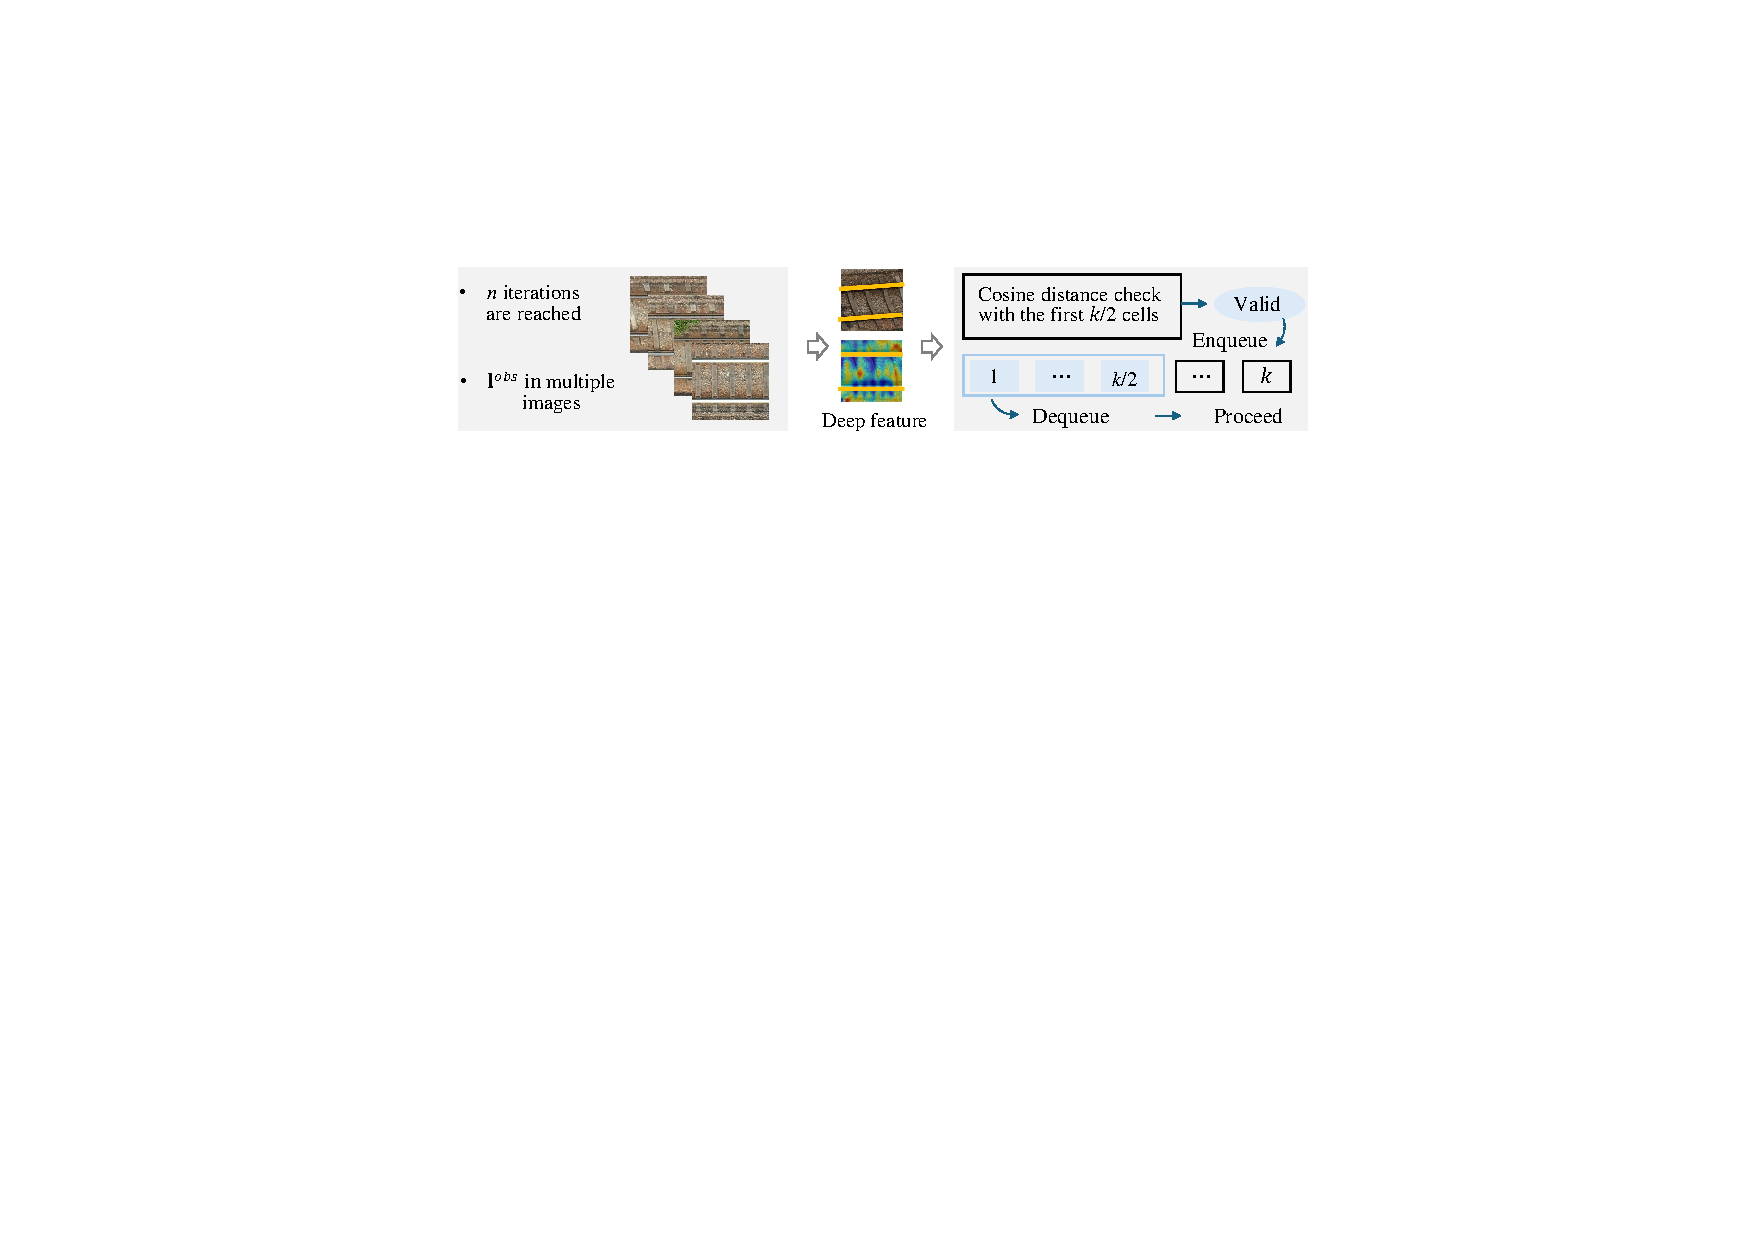
\includegraphics[width=0.98\textwidth]{images/visualCheck.pdf}
    \caption{Visual alignment check in Kalman Filter.
    We project the estimation of \rlp in multiple images and extract the deep feature with pre-trained network.
    Then, 
    we check their cosine distance with the first $n/2$ cells in the queue,
    where $n$ is obtained by dividing the \rlp width by the step size $t$.}
    \label{fig_visualCheck}
\end{figure}

For each seed of \rlp~,
we will track it with the Kalman filter and terminate the track when one of the following conditions is met.
(1) \textit{Overlap}:
with each of the last $k$ \rlp~ in the current filter process, 
we find the nearest \rlp~ set that have been reconstructed in the previous filter process.
If half of the \rlp~ can find a nearest one within $\frac{1}{10}d$,
we say that the overlap has occurred.
(2) \textit{Inaligned deep features:}
the texture is not aligned with the previous state,
We save the set of deep features that has passed the texture validation in a queue and use the first half of the elements in the queue to validate the new $\left\{\mathbf f^\prime\right\}_{i=1}^{m1}$:
\begin{equation}
\sum_{i=1}^{m_1} \mathbb{I} \left( \exists j \in \left[ m_2 \right], \, \cos \left( \mathbf{f}_i, \mathbf f^{\prime}_j \right) > \theta \right) \geq \frac{m_1}{2}
\label{eq_featureValidation}
\end{equation}
where $m2$ is the total number of $\mathbf f$ in the first half of the feature set in the queue;
$\mathbb{I}$ represents an indicator function which takes the value of 1 when a certain condition is true and 0 otherwise.
If $\left\{\mathbf f^\prime\right\}_{i=1}^{m1}$ satisfies \cref{eq_featureValidation},
it is pushed to the queue, 
and then the queue is dequeued if its cell passed $cal$.
(3) \textit{Degenerate reconstruction:}
there is no correct 3D line that can be reconstructed from multiple images in \cref{sec_linereconstruction}.
Note that
it is unnecessary to check for termination in every estimate, especially when we use a small $t$ for robustness;
instead,
we employ this check when $k$ iterations are reached and roll back to the state of the previous check when the overlap or feature inconsistency occurs. 

\begin{figure}[htbp]
    \centering
    % 第一个子图
    \subfloat[The weight function of \cref{eq_gradientweight}]{
        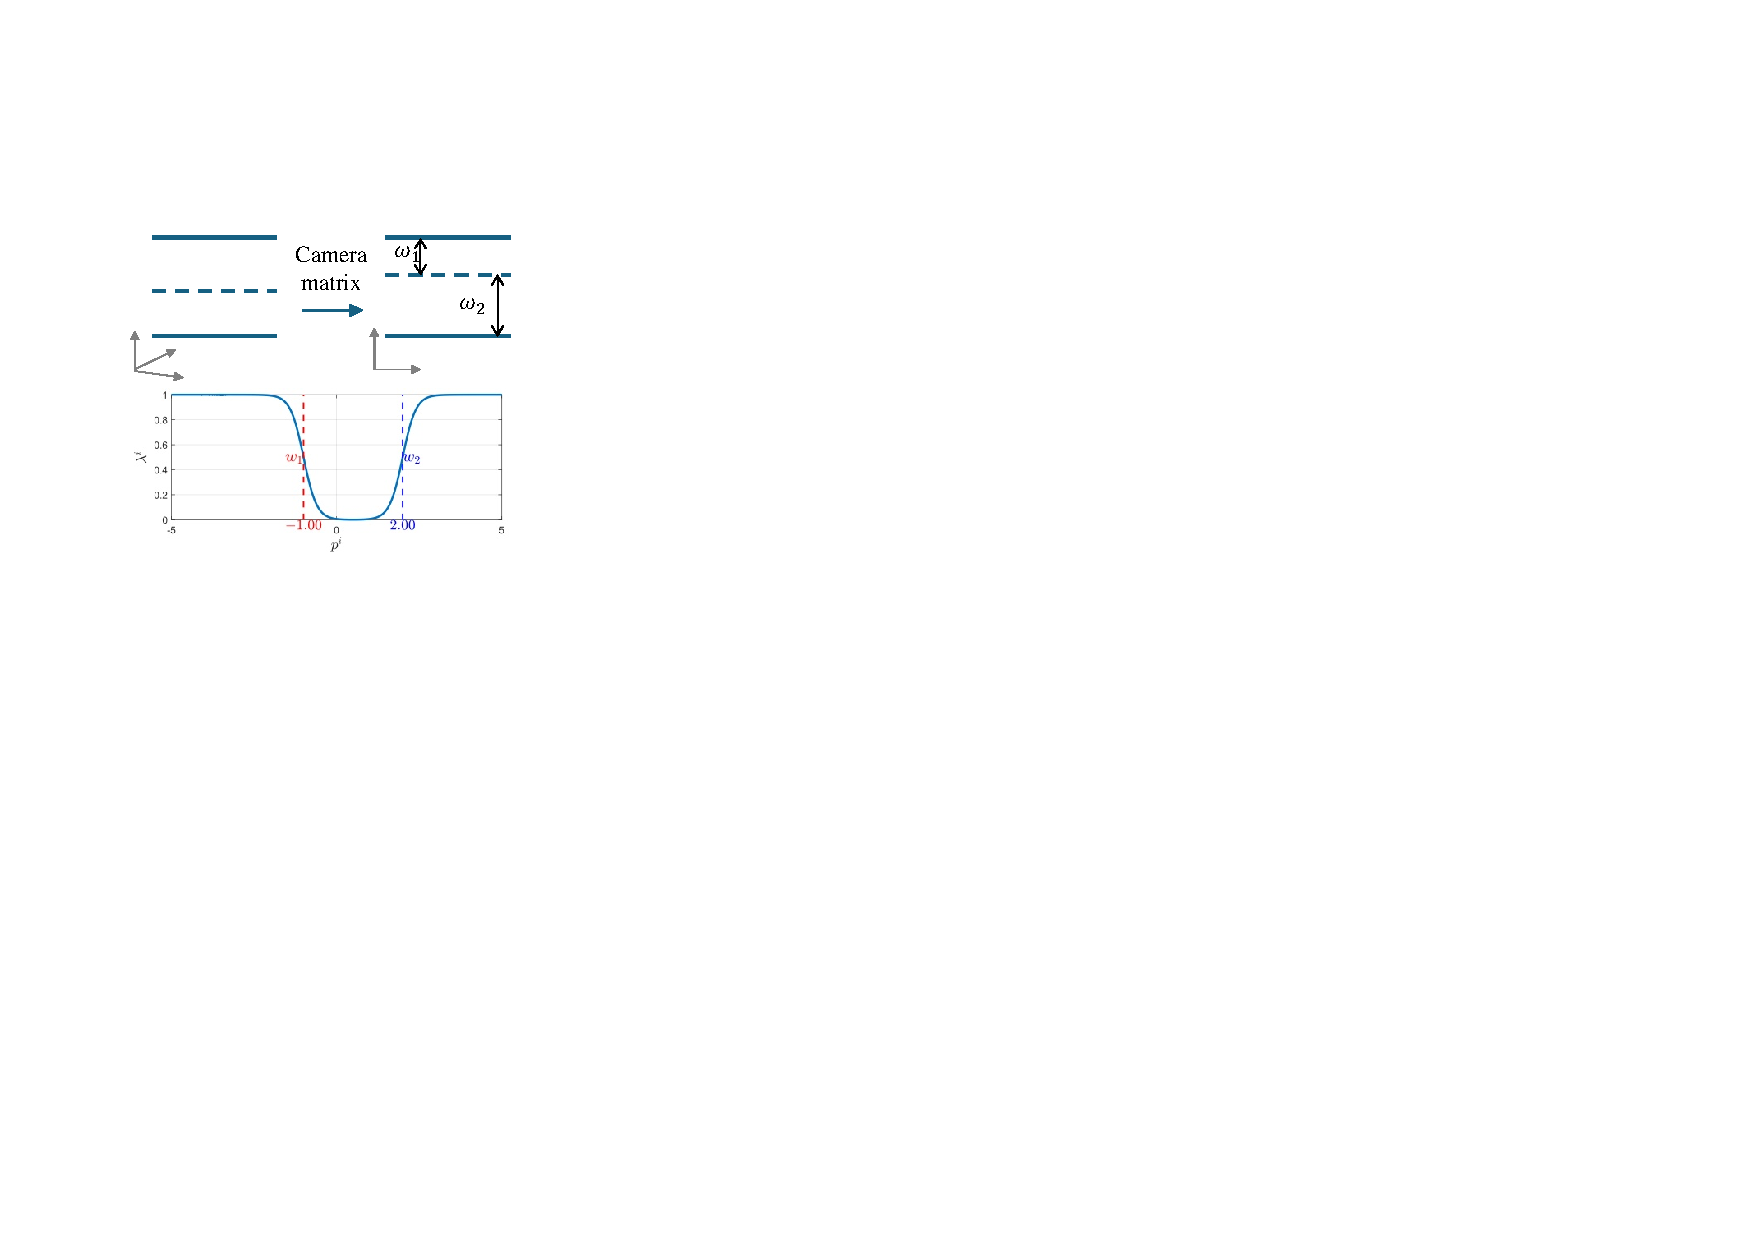
\includegraphics[width=0.24\textwidth]{images/linereconstruction1.pdf}
    }
    \hfill % 空格,均匀分布
    % 第二个子图
    \subfloat[Some results of the GD algorithm]{
        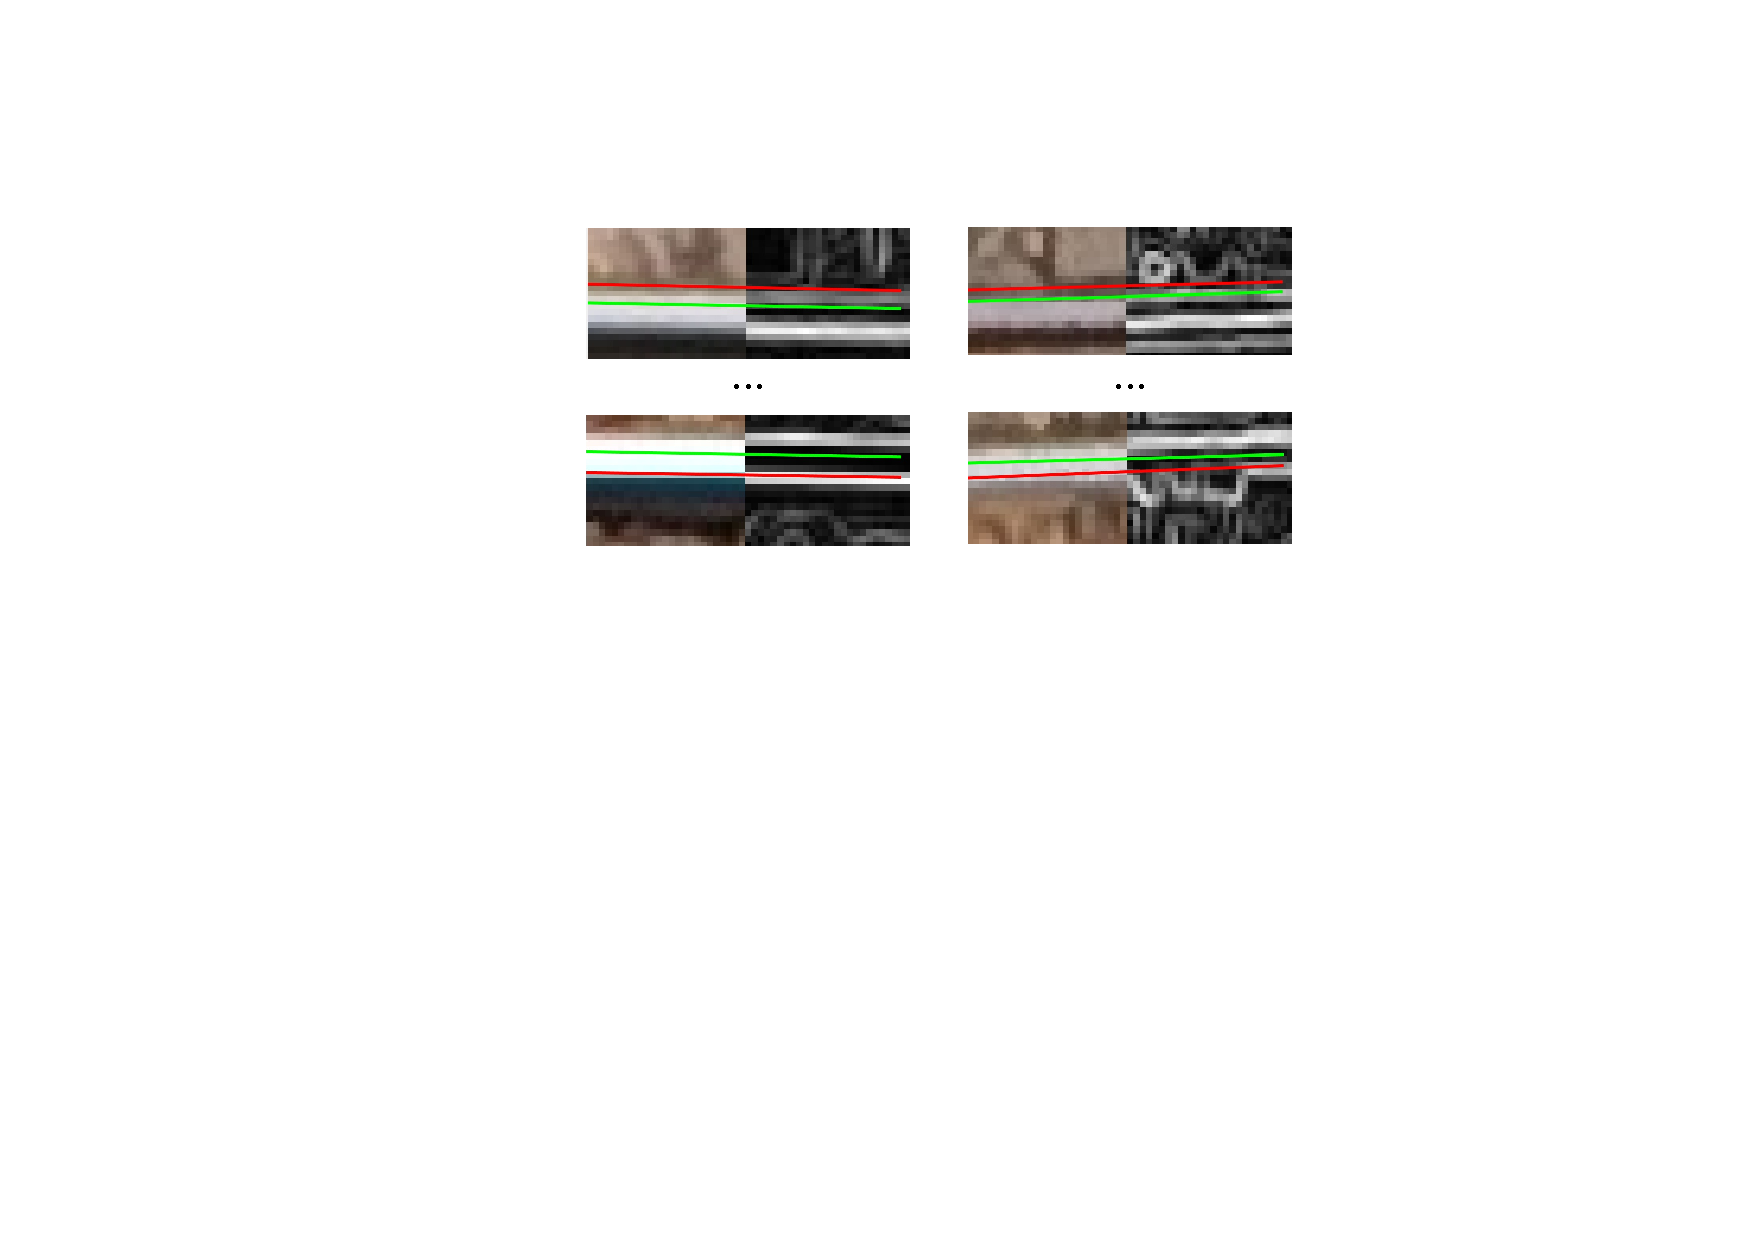
\includegraphics[width=0.44\textwidth]{images/linereconstruction2.pdf}
    }
    \hfill
    % 第三个子图
    \subfloat[The 3D lines from image pairs]{
        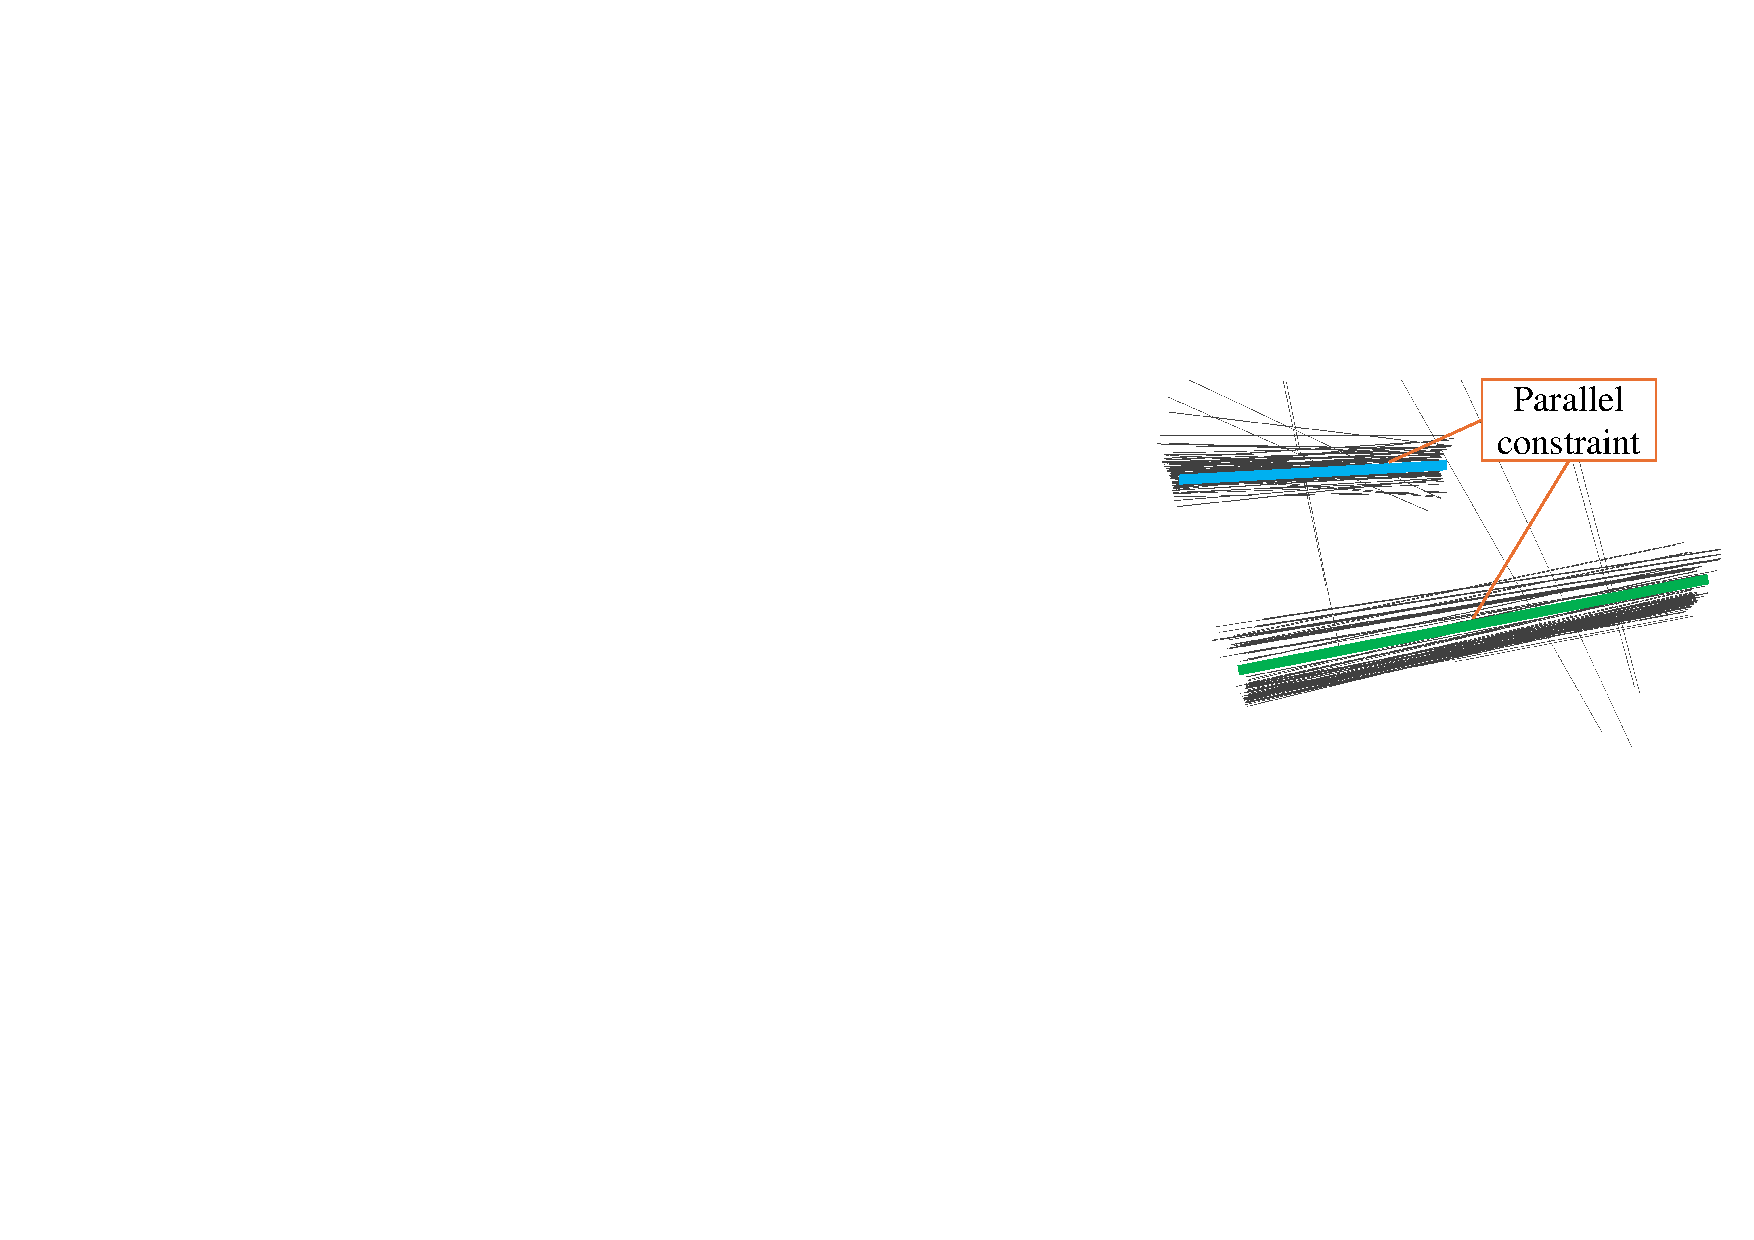
\includegraphics[width=0.25\textwidth]{images/linereconstruction3.pdf}
    }
    \caption{Illustration of the line reconstruction.} % 总标题
    \label{fig:three-images}
\end{figure}


\subsection{Accurate railway line position with gradient descending}
\label{sec_linereconstruction}
For a 3D line in $\mathbf{x}^{pre}$~(\cref{eq_statetransition}),
we convert it into image with camera matrix and obtain the 2D line segment
$\mathbf{l}^{pre}=\begin{bmatrix} x_c,y_c,\theta \end{bmatrix}$;
then we search around $\mathbf{l}^{pre}$ for the observation $\mathbf{l}^{obs}$,
which should have the maximum gradient response:
\begin{equation}
 \mathcal{L} = \sum_{i=1}^{N} \lambda_i \cdot \|G_x \left(x_i, y_i \right),G_y\left(x_i, y_i\right) \|^2, 
\label{eq_GDobjfunction}
\end{equation}
where $G_x$ and $G_y$ is the gradient magnitude in two dimensions;
the sample point is calculated by
\begin{equation}
\begin{bmatrix}
x_i \\
y_i
\end{bmatrix}
=
\begin{bmatrix}
x_c \\
y_c
\end{bmatrix}
+
\begin{bmatrix}
\cos\theta & -\sin\theta \\
\sin\theta & \cos\theta
\end{bmatrix}
\begin{bmatrix}
h_i \\
p_i
\end{bmatrix},
\label{eq_samplepoints}
\end{equation}
where $h_i$ and $ p_i$ is the parallel and horizontal distance to $\mathbf{l}^{obs}$,
respectively.
Because the \textit{RL} has a width that is different at with positions and images,
we use $\lambda_i$ in \cref{eq_GDobjfunction} to weight the gradients:
\begin{equation}
\lambda_i= 1 - \frac{1}{1 + e^{10\left(w_1-p_i \right)}} + \frac{1}{1 + e^{10\left(w_2-p_i\right)}}
\label{eq_gradientweight}
\end{equation}
where $w_1$ and $w_2$ are the distance calculated from the the prior width of \textit{RL}.

We use the gradient ascend to find $\mathbf{l}^{obs}$ with \cref{eq_GDobjfunction}:
\begin{equation}
\mathbf{l}^{obs}_{i}=\mathbf{l}^{obs}_{i-1}-\alpha \Delta \mathcal{L},
\label{eq_gditerative}
\end{equation}
where \( \alpha \) is the learning rate.
\( \Delta \mathcal{L} \) is the gradient from \cref{eq_GDobjfunction} and \cref{eq_samplepoints}:
\begin{equation}
\Delta \mathcal{L} = - \sum_{i=1}^{N} \lambda_i \mathbf{J}_i
\begin{bmatrix}
G_x(x_i, y_i) &
G_y(x_i, y_i)
\end{bmatrix}^{\top},
\end{equation}
where $\mathbf{J}_i$ is the Jacobian matrix
\begin{equation}
\mathbf{J}_i=
\begin{bmatrix}
\partial x_i / \partial x_c & \partial x_i / \partial y_c & \partial x_i / \partial \theta \\
\partial y_i / \partial x_c & \partial y_i / \partial y_c & \partial y_i / \partial \theta
\end{bmatrix}^{\top}
\end{equation}
\cref{eq_gditerative} takes $\mathbf{l}^{pre}$ as input and iterates until the parameters converge, i.e., when the change in the parameters is smaller than a predefined threshold.

In the task of reconstructing the optimal 3D line segment from multiple $\mathbf l^{obs}$, we propose an efficient strategy. 
Specifically, 
for \( n \) images with \( n \) observed line segments, 
we first perform pairwise 3D line segment reconstructions for all image pairs, 
generating \( n \times (n-1) / 2 \) candidate 3D line segments. 
Next, a score is computed for each 3D line segment by calculating the weighted sum of distances to other 3D line segments within a specified distance threshold. 
Finally, the 3D line segment with the highest score is selected as the optimal reconstruction.
We say the degenerate reconstruction occurs when the highest score is 0 and the Kalman filter will be terminated as illustrated in  \cref{fig_kalmanflow,fig_visualCheck}. 
Using the known RLP structure, 
we can easily use the approximate RLP width range to define an appropriate inlier threshold,
enhancing the robustness and accuracy of the method.


    








